\chapter{Research}
\label{chapter:research}

This chapter documents the research that was completed prior to the development of the application. Research was undertaken to determine the scope of the project, the technologies to be used, and the desired outcome. The outcome of the research was used to examine the possible challenges of this project, including any problems that may be encountered by choosing one technology over the other.

% This section outlines some reading you have done in this field, organised by ideas, research trends.
% Have you found similar software that inspires your system?
% Objective of this chapter is to tell the reader that this is an important and interesting problem, other people have done work on it before, and this is inspiring your development.

\section{Background Research}
% Research related to identifying the problem this project solves, research into solution definition

Web-based applications are becoming increasingly popular as the web develops; they are often favoured over traditional desktop applications when it comes to activities such as writing documents (Google Drive, Office Live) or backing up files.\cite{6068340} Desktop applications will often require downloading large installation files, dependencies (Java, .NET), and can often be limited to a single platform. Web apps are now becoming the norm, as they are far more flexible, can be updated or distributed instantly and are almost entirely cross platform.\cite{5936687}

According to Taivalsaari and Mikkonen, ``Towards the end of this decade, the Web will become the dominant platform for the majority of 
end user software''.\cite{6068340} It's only a matter of time until game engine suites such as Unity\cite{unity}, CryEngine\cite{cryengine} and Unreal Engine\cite{unreal} adapt to the web. Creating a web application in this area now will make it easier for new game developers to get started on building games without having to download software. This also eases game publishing significantly by allowing users to publish their games instantly to the cloud with a single click.

WebGL is an open-source API for rendering 2D and 3D graphics in the browser, which is based on OpenGL ES; a commonly used graphics processing API that powers 3D graphics on the iPhone, iPad and Android devices.\cite{parisi2012webgl} WebGL is quickly becoming ``the new standard for 3D graphics on the Web''\cite[p2]{parisi2012webgl} as it is the most powerful and flexible way to render graphics in-browser without any extra dependencies or plugins needed. The JavaScript programming language is used to access the WebGL API, which can be rather complicated to program with; ``To do anything more than the most basic tasks using [WebGL] out of the box requires serious effort and literally hundreds of lines of code.''\cite[p44]{parisi2014programming}

The solution to the WebGL API's complexity is to use a library that wraps it and simplifies the interface. The Three.js\cite{threejs} JavaScript library accomplishes this by providing easy to use classes such as models, lighting, scenes and cameras. ``A program written in raw WebGL style using hundreds of lines of code can be expressed in just a few dozen lines of code with Three.js.''\cite[p57]{parisi2014programming} While Three.js greatly simplifies the process of rendering scenes in the browser, it's not good enough for the development of games, as it only provides a framework for rendering scenes without any game logic.

The architecture of the game engine is critical to how accessible it is to developers. The Entity-Component-System is a pattern that can simplify how game objects are defined by separating behaviour into smaller components. Each empty game object can be made up of many components, which will add up to produce a dynamic and interesting object, for example; a blank `cube' object could have a model component, giving it something to render, and a physics component which will allow it to collide with the world and other physics objects.\cite{gregory2014game} This pattern essentially reduces game objects from what would normally be a class inherited from a base object, to a list of components and properties.

An ECS-based game engine with an integrated editor will give users the power to build games even with minimal programming knowledge. A good example of this is Unity, which allows users to build their games just by creating their scene, adding entities such as a floor, and adding physics components to those entities.\cite{unitycreatingscenes} Adding a controller such as the `First Person Controller' to their project allows the player to input and explore the scene just like in a standard first person shooter game.\cite{unitycharactercontrol}

\section{Alternative Existing Solutions}
\subsection{Unity}
Unity is a 3D game engine with an integrated editor and a huge online library full of assets such as models, sounds and various scripts or tools. Unity is a cross-platform engine that is used on Windows, Linux, Mac OSX, mobiles (Android, iOS, Windows, BlackBerry), consoles (PS3, Xbox360, Wii U) and even in browsers.\cite{unity}

Unity's ability to publish games to the web via the Unity Web Player browser plugin make it a powerful solution to creating games for the web. The only downside to the web player is that the user must install the runtime plugin to be able to play.\cite{unityweb}

The Unity game engine is based on the Entity-Component-System pattern, with the majority of components used being supplied by the engine (Such as lighting, physics, models).\cite{unitycomponents} Unity games can be scripted in one of three languages; C\#, Boo or JavaScript.

The Unity scene editor allows complex entities to be created simply by adding a number of components to an empty entity from a list. The properties for each component can then be edited in the \emph{properties inspector}, such as changing the model or colour of an object. \cite{unitycreatingscenes}

% Add pic of inspector

\subsection{PlayCanvas}
\begin{quote}
PlayCanvas is a visual development platform for 3D web content. Both the tools and the web apps you build are powered by HTML5. The entire software platform is web hosted so there's nothing to install and you can access your work from any device that runs one of the supported web browsers.\cite{playcanvas}
\end{quote}

PlayCanvas features the ability to publish games, fork public and example projects, collaborate with multiple users and sync project files to GitHub. The game engine is based on the Entity-Component-System pattern, with several components being provided for building simple games out of the box, and support to create new scripted components using JavaScript.\cite{playcanvas}

The PlayCanvas game editor features impressive real-time collaboration with multiple users, however it only has features intended for scene editing. The user must leave the editor to manage their project for simple tasks such as editing scripts, syncing to GitHub, and publish their project.

\subsection{CopperLicht}
\begin{quote}
CopperLicht is an open source WebGL library and JavaScript 3D engine for creating games and 3D applications in the webbrowser. It uses the WebGL canvas supported by modern browsers and is able to render hardware accelerated 3d graphics without any plugins.\cite{copperlicht}
\end{quote}

The CopperLicht game engine uses an OOP style approach to the architecture of a game, with entities being defined via scripting rather than by selecting a group of components as Unity does. The CopperLicht engine will handle rendering, physics and animations, any extra functionality must be added manually by the user with a script.\cite{copperlichtfeatures}

The CopperLicht world editor, \emph{CopperCube} is an editor designed to create the worlds used in a CopperLicht game. It works by generating a scene file which is loaded by a HTML file, generated Android APK, Windows EXE or Mac OSX App.\cite{coppercubefeatures} Actions and behaviours can be added to the game by JavaScript scripting, or by using predefined behaviours defined in CopperLicht such as `Fly in a Circle'.\cite{copperlichtbehaviours}

\subsection{Comparison of Solutions}
A comparison of Stratus and alternative solutions has been performed, comparing the features available. The results of this comparison are visible in Table \ref{tab:solutions}. The features compared are: Built-in version control (VC), Supports Git usage (Git), Real-time collaboration (Real-time), Conglomerated editor features such as scripting (Editing), Entity-Component System architecture (ECS), Built-in forking of example or public projects (Forking) and one-click publishing (Publish).

\begin{table}[H]
	\begin{tabular}{| l | c | c | c | c | c | c | c |}
	\hline
	& VC & Git & Real-time & Editing & ECS & Forking & Publish\\\hline
	Unity 		& \ding{56}	& \ding{52}	& \ding{56}	
				& \ding{52}	& \ding{52}	& \ding{56}	& \ding{56}\\\hline
	PlayCanvas 	& \ding{56}	& \ding{52}	& \ding{52}	
				& \ding{56}	& \ding{52}	& \ding{52}	& \ding{52}\\\hline
	CopperLicht & \ding{56}	& \ding{52}	& \ding{56}	
				& \ding{56}	& \ding{56}	& \ding{56}	& \ding{56}\\\hline
	Stratus & \ding{52}	& \ding{52}	& \ding{56}	
				& \ding{52}	& \ding{52}	& \ding{52}	& \ding{52}\\\hline
	\end{tabular}
	\caption{Comparison of alternative solutions.}
	\label{tab:solutions}
\end{table}

The comparison reveals that many of the examined alternative solutions have areas that could be improved upon. For example, Unity has a strong engine and editor but has no methods for quick publishing of created games, apart from third party websites.

\section{Technologies}
\subsection{Web Application Hosting}
\paragraph{Criteria.}
This project requires a powerful and scalable hardware solution, with automatic load balancing and ease of deployment being the most important requirements. The ability for the hosting solution to scale with the application and how many users there are will be essential in the future of the project.

\paragraph{Dedicated Server.}
The first option is to use a dedicated server without any distributed computing or virtualization. For this case I would use my own server which is provided by Hetzner; a Root Server EX40. As I would be using my own server, this option would be the most cost-effective, however the performance and scalability of the platform would not be suitable enough for the final release of the project.

It would be possible to make this option viable by manually setting up load balancing with nginx and caching tools such as memcached, however the workload to install and configure these systems correctly would be superfluous.\cite{nginxloadbalancing,memcached}

\paragraph{Amazon Elastic Compute Cloud.}
Amazon Elastic Compute Cloud (EC2), part of the Amazon Web Services (AWS) collection, is an \emph{Infrastructure as a Service}.\cite{awsec2} It is used by hundreds of large companies to host their web applications or even game servers. EC2 provides scalable virtual servers which can be made to fit any requirement by allowing the developer to install the required operating system and any type of application needed.

EC2 provides the flexibility, scalability and power needed for this project by automatically scaling up and down EC2 instances as needed.\cite{awsec2} Load balancing can be achieved using the Elastic Load Balancing service provided by Amazon.\cite{elasticloadbalancing} The only downside to using EC2 is that each EC2 instance will require setting up and deploying which could increase the workload significantly.

\paragraph{Amazon EC2 Container Service.}
Amazon EC2 Container Service (ECS) brings EC2 one step further by making deployment as simple as possible. Docker.io \emph{dockerfiles} are used to automatically create EC2 instances based on a specification created in a simple text file.\cite{awsecs} These instances can then be populated with apps and data specified in the dockerfile.\cite{dockerfile}

Using ECS would significantly speed up the time required to set up the necessary EC2 instances, especially if multiple instances are required; such as a load balancer, application and a database. ECS is currently in a preview state which must be applied for, so it may be unusable for this project unless the state of this changes.

\paragraph{Heroku.}
Heroku is a \emph{Platform as a Service} web application platform for deploying scalable web apps in the cloud. Heroku will automatically scale and manage applications deployed on the platform, making sure the application performs perfectly even under stress.\cite{heroku} Heroku has support for deploying applications built in many languages including Java, Node.js and Python.

Heroku itself has no storage systems available apart from their PostGRES database service. The lack of integrated file storage may complicate the implementation of user project storage. A cloud storage service such as Amazon S3 must be used instead.

\paragraph{Amazon Elastic Beanstalk.}
Amazon Elastic Beanstalk is a web application deployment service similar to Heroku. Elastic Beanstalk takes a web app and deploys it to an EC2 instance, automatically setting up and managing load balancing, scaling and any capacity needs.\cite{awselasticbeanstalk}

Using Elastic Beanstalk in my project would make deployment quick and painless, while still maintaining the same level of control that a standard EC2 instance has. The automatic load balancing process used with Elastic Beanstalk will automatically generate multiple instances of the application as needed so it can always be available no matter how many users are accessing it without any manual management.

\subsection{Web Application Frameworks}
\paragraph{Criteria.}
The web application framework should be as lightweight as possible, allowing the application to scale as needed. The framework should be flexible in use and support the Model-View-Controller pattern to be used in development. A strong template engine should be available to allow dynamic front-end pages to be built efficiently.

\paragraph{Node.js.}
Node.js is a platform for building applications using JavaScript as the main language. It uses Google's V8 JavaScript engine to increase the performance of JavaScript by compiling standard JavaScript to machine code.\cite{nodejs}

By default, Node.js isn't a web application framework, but can be made into a powerful one using one of many libraries available on the Node Package Manager.\cite{npmjs} An example of this would be using the lightweight Express web framework library and a template engine such as EJS or Jade.

\paragraph{Django.}
Django is a web application framework built on Python, which uses an MVC-like approach to designing websites.\cite{django} Django is designed to allow common web development tasks to be completed quickly and easily. It does this by providing APIs for Object-Relational Modelling to ease database usage, a powerful templating engine and automatic administration interface generation.\cite{djangooverview}

While Django makes complex web application development simple, it is bloated with features that may not be used at all in a lot of projects. For the purpose of creating this project, Object-Relational Modelling and automatic administration page generation may be entirely unused. 

\paragraph{Flask.}
Flask is lightweight Python-based web application microframework that comes only with a server and a templating engine. Flask is designed to be relatively simple at it's core, but becomes powerful through the use of modules that add extra functionality if needed.\cite{flask} The simplistic nature of Flask means it can be up and running relatively quick compared to other frameworks.

\subsection{Project Storage}
\paragraph{Criteria.}
User project storage is an extremely important part of this project. How the projects are stored will define how the application performs while saving projects, serving project files to players, and managing how users will collaborate on projects.

The project storage medium should be able to support some kind of version control, have good read/write performance, and should be scalable to some extent.

\paragraph{GitHub API.}
Storing user projects via the GitHub API without any server-side storage was the original proposed approach for this project.\cite{githubapi} Integrating the GitHub API into this project can allow the user to log into the application using their GitHub credentials via the GitHub OAuth system. \cite{githuboauth} This will provide an easier form of authentication than storing user details and passwords in a database which may not be as secure.

All storage can be performed directly through API requests to GitHub by submitting the user's files without any storage on the server.\cite{githubapicommit} This provides both version control and the cloud-based user storage this project requires, however access to the API is depended on heavily, which may be unavailable or slow at times.

There are a few problems with this approach. First is that it is very volatile; changes made by the user may be discarded if the user leaves the page without committing. Secondly, using the GitHub API does not do any merging of files, but instead overwrites files entirely, making collaboration hard for the users. This is discussed in greater detail in the Prototyping and Development area of this report (Section 6).

\paragraph{Amazon Elastic Block Storage.}
Amazon Elastic Block Storage (EBS) is a scalable solution to storage for use on Amazon EC2 instances. Performance on EBS is very high, as there are options for selecting between high/normal performance SSDs and standard hard drives. EBS volumes can be mounted directly to EC2 instances allowing standard file storage without any APIs.\cite{awsebs}

While EBS has no form of version control, local Git repositories could be used to manage version control. Since EBS can be mounted directly onto an EC2 instance, the command-line Git tool can be used to directly perform Git operations such as committing or even pushing to a remote server such as GitHub. Using GitHub with this option also means collaboration between users may be possible.

Implementing load balancing while using a mounted storage such as this may be problematic, since EBS volumes may only be mounted on a single EC2 instance. A workaround to this would be to use a single instance to write to the disk and then connect to that from the load balancing instances.

\paragraph{Amazon Simple Storage Service.}
Amazon Simple Storage Service (S3) is a storage system that is accessible through a REST-like API, which can be used with the AWS SDK which is available for several languages.\cite{awss3} S3 stores data as objects inside a container called a \emph{bucket}, where buckets can store any number of files up to 5GB each.

S3 is a powerful and cost-effective storage medium, especially suited to content delivery. It's backup and version control systems make it fairly suitable for this project.\cite{awss3} It may be hard to implement other systems like Git for user project storage and collaboration on S3 since buckets are only accessible via an API.

\paragraph{MongoDB GridFS.}
MongoDB GridFS is a high performance file system based on the MongoDB document database. It is designed to be used when documents that are larger than 16MB are to be stored in a MongoDB database, but can be used for small documents for consistency without any significant performance loss.\cite{gridfs}

Because GridFS is based on MongoDB, it is extremely suitable for horizontal scaling, but it does not support any atomic operations.\cite{gridfsatomic} The lack of atomic operations could make collaboration and version control hard to implement.

\subsection{Alternative Scripting Languages}
\paragraph{Criteria.}
Alternative browser-based scripting languages could be used to add typing and Object Oriented Programming to the game engine and user made games. While JavaScript has limited OOP functionality (Prototype chaining for inheritance), it is still a valid choice.

\paragraph{TypeScript.}
TypeScript is another alternative to JavaScript that was created by Microsoft to replace JavaScript. It provides a strong level of OOP functionality, scalability for large projects and optional type declarations on top of standard JavaScript syntax.\cite{typescript} In order to use existing JavaScript libraries with TypeScript, a header file is required to make the functions visible to TypeScript. TypeScript is transcompiled directly to JavaScript, and because of this it will often perform just as well as JavaScript does and doesn't require a virtual machine.

\paragraph{Dart.}
Dart is a compiled JavaScript alternative created by Google, with it's own virtual machine that supports OOP principals and static typing. Dart can also be transcompiled to JavaScript which allows dynamic loading of either the Dart file or the JavaScript file depending on what is supported by the browser.\cite{dart} Dart supports interaction with standard JavaScript libraries such as jQuery without needing to be modified in any way.

Dart runs in it's own Dart VM which boasts huge performance gains over JavaScript virtual machines, however the Dart VM is currently only supported on the \emph{Dartium} browser; a branch of Google Chrome. When using other browsers such as Firefox or the standard version of Chrome, Dart code transcompiled to JavaScript will often perform worse compared to standard JavaScript.\cite{dartperformance}

\subsection{JavaScript Libraries}

\paragraph{Rendering.}
Alternatives to Three.js were examined to determine their suitability to the project. The rendering library used should be suited to use in game development and have a flexible API.

SpiderGL is a WebGL wrapper that does very little abstraction to the API, making using WebGL slightly easier while still having low level objects such as vertex buffer objects.\cite{spidergl} In comparison to Three.js, SpiderGL lacks a lot of features for rendering complex scene components, as well as being significantly harder to use.

SceneJS is a rendering library for JavaScript suited towards visualising highly accurate scenes with large amounts of detail similar to Computer-Aided Design (CAD). This library can be used to create and explore medical or engineering recreations, for example; the human body.\cite{scenejs}

\paragraph{Physics.}
Existing research completed by Yogya and Kosalaa determined that out of several possible JavaScript physics engines including Bullet, Cannon and JibLib, ``Bullet is the best physics framework to be integrated into the WebGL-based game engine''.\cite{yogya2014comparison} Their conclusion is based on several factors, including performance, accuracy and compatibility with multiple browsers. The Bullet Physics library has been ported to JavaScript under the name `Ammo.js'.

% todo: ref ammo.js

\paragraph{Web Audio.}
Research into the use of audio in JavaScript has proven that the W3C Web Audio API is a sufficient option for this project's requirements. The Web Audio API supports the use of Cartesian coordinates to project sound effects using binaural positioning in a 3-Dimensional environment.\cite{webaudio} Binaural positioning is crucial to establishing the atmosphere in games such as first person shooters; where directional audio is necessary to create a sense of immersion.

The Web Audio API has support for real-time DSP sound filtering effects, which could be useful in the production of a game. DSP filters could be used to add distortion to ambient sounds based on events in the game such as an explosion.

Real-time audio can be examined in-detail with the Web Audio API using an audio analyser, which outputs a Fast Fourier Transform table (FFT). This table contains a set of volumes at specific frequencies. Games could be built around analysing these frequencies and performing specific actions, for example: triggering rendering effects when music becomes particularly intense.

\section{Other Relevant Research}
\paragraph{WebGL Usage.}
I have used WebGL in the past to create a simple rendering application. My experience with using WebGL was comparable to how it is mentioned in \emph{Programming 3D Applications in HTML5 and WebGL}\cite{parisi2014programming}. The application was designed to render objects using the pure WebGL API through JavaScript without any wrapping libraries. The result was an application of exactly 400 lines that was only capable of rendering a single multi-coloured box as seen in Figure \ref{fig:webgl} - this alone is evidence of how difficult WebGL can be to use.

\begin{figure}[h]
	\centering
	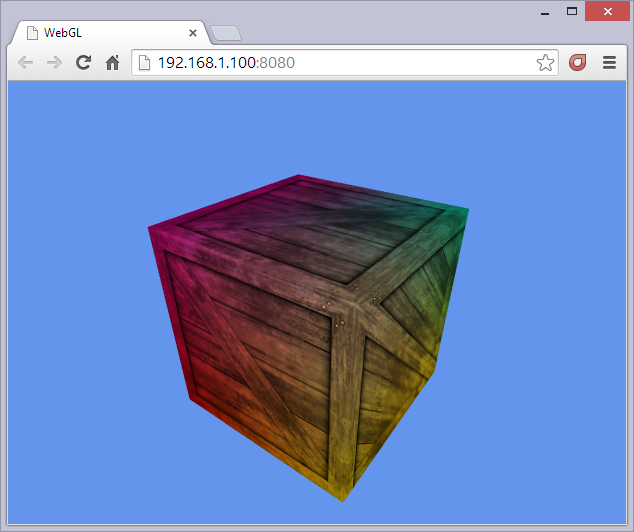
\includegraphics[scale=0.5]{webgl}
	\caption{A textured cube rendered with WebGL}
	\label{fig:webgl}
\end{figure}

This experience using WebGL was the origin of my idea to simplify the method for developing games using WebGL. WebGL has great potential as the foundation for a powerful game engine, with it's strengths becoming evident while using OpenGL's shader language GLSL. Though it is powerful, the workload associated with using WebGL for even a small application was excessive.

\paragraph{GitHub API Concept Application.}
A concept application was created to explore the plausibility of using the GitHub API for project storage, version control and collaboration. The application was developed using Flask, JavaScript and the Python 3 libraries urllib and json. The interface of the application can be seen in Figure \ref{fig:proto1}.

\begin{figure}[h]
	\centering
	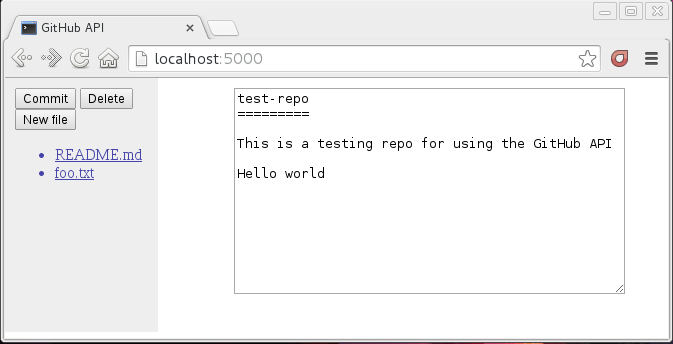
\includegraphics[scale=0.6]{proto1}
	\caption{GitHub API concept application}
	\label{fig:proto1}
\end{figure}

The functionality implemented in the concept application included creating or deleting files in the repository, modifying the content of files and committing the changes that were made.

The process of creating and pushing a commit using the GitHub API involves 5 steps, as observed by Matt Swanson\cite{githubapicommit}:
\begin{enumerate}
	\item Retrieve the hash value of the latest commit.
	\item Retrieve the hash value of the tree in the commit.
	\item Create a new tree, based on the current one. This will store the changes in the commit, such as file contents.
	\item Create a new commit pointing to the new tree.
	\item Submit the new commit as the HEAD reference, which will change the latest commit to the new one.
\end{enumerate}

From developing this concept application I was able to determine that the GitHub API was not suitable for the needs of this project. The process of committing a file through the API severely limits collaboration methods by overwriting changes entirely; no merging of changes will happen unlike the standard usage of Git. The GitHub API was also rather slow to access, taking up to 10 seconds to complete a commit.

\section{Resultant Findings \& Requirements}
Based on the research completed, the following requirements have been determined, including optimal choices for technologies and architectures that will be utilised in this project.

\subsection{Background research.}
The background research has shown that web applications are becoming the standard, with almost every type of application now being able to be created on the web. Applications built on the web greatly simplify the process that users go through to access and utilise an application, and with cloud storage being utilized; the user doesn't need to store any files locally.

Game engines are being made easier to use and understand by patterns such as the Entity-Component System. This system builds game objects by aggregating functionality from several smaller components, without any actual functionality being made specific to the object.

\subsection{Existing Solutions.}
A comparison of the existing solutions to this problem has revealed that alternative solutions can be improved upon by aggregating functionality including version control, git usage, collaboration, entity-component system based game engine, integrated editor controls for scripting and project management, forking existing projects and one-click publishing of projects. While solutions such as PlayCanvas provide a more interactive approach with real-time collaboration, my solution of using Git is a valid choice as many developers will be more familiar with it.

\subsection{Technologies.}
\paragraph{Web Application Hosting.}
An analysis and comparison of the examined application hosting solutions has determined that Amazon's Elastic Beanstalk service would be the optimal choice for hosting the web application, with Amazon EC2 Container Service being the second choice.

Elastic Beanstalk has several strengths over the other options, with the most pronounced being the automatic load balancing and interaction with EC2 instances. While other hosting solutions such as Heroku do have load balancing, they do not have the huge library of web services that can can be integrated with like AWS does.

The EC2 Container Service was a close second to Elastic Beanstalk, giving the most control over how the application would be deployed, but would require setting up the Amazon Elastic Load Balancer to interact with the containers manually.

\paragraph{Web Application Framework.}
The examined frameworks for developing web applications were fairly similar in functionality, flexibility and scalability. In my opinion, the optimal application framework to use would be Flask, as it requires minimal setup and can be extended using modules as needed. The other examined frameworks; Django and Node.js were too feature-heavy and required extra setup time respectively.

\paragraph{Project Storage.}
For user project storage, based on the findings the optimal project storage solution would either be Amazon S3 or Amazon Elastic Block Storage.

S3 provides an API for storing and retrieving files, with a version control mechanism. This could provide all of the functionality needed for project storage, however using S3 could make implementing collaboration difficult compared to using Git for version control and collaboration. Using S3 with the load balancing would be straightforward, as S3 can be accessed from multiple sources at once through the API.

Elastic Block Storage, which is a simple mounted volume which could be used with Git to provide a means of version control and collaboration. Using EBS with load balancing software is fairly challenging however, as the volume can only be mounted on a single application instance and load balancing will generate multiple instances of an application.

\paragraph{Alternative Scripting Language.}
Alternative scripting languages, Dart and TypeScript, were examined and compared to JavaScript. As the alternatives require compilation/transcompilation, standard JavaScript was decided as the optimal choice for use in this project. Implementing transcompilation in the web application is unnecessary as standard JavaScript can be used without major loss of functionality.

\paragraph{JavaScript Libraries.}
As a result of the research into several rendering libraries based on WebGL, Three.js was determined to be the most suitable for this project, as it has the features, flexibility, stability and optimisation needed for use in game engines. The API it provides is abstracted significantly from the WebGL API to provide simple methods for doing normally complex tasks.

The Bullet physics engine and Web Audio API are highly suited for use in this project as explored in the research, providing functionality that is crucial for use in game engines.


% todo
% other research done
% Using Threejs
% Ammo.js for Bullet in JS
% Choosing a simple database for storing a list of published games
% 	Why AWS DynamoDB wasn't used etc
% 	

% todo
% Change from ECS to EC2, why